\documentclass{beamer}
\usepackage[utf8]{inputenc}
\usepackage{ifpdf}
%\usepackage{hyperref}
\usepackage[english]{babel}
\usepackage{amsfonts}
\usepackage{amsmath}
\usepackage{amsthm}
\usepackage{color}
\usepackage{graphicx}
\usepackage{tikz}
%\usepackage{multicol}
%\usepackage{moreverb}
\usepackage{listings}
%\usepackage{color}
%\usepackage{algorithm}
%\usepackage{algorithmicx}
%\usepackage{algpseudocode}
%\usepackage{longtable}
%\usepackage{geometry}
%\geometry{margin=2cm}
%\floatname{algorithm}{Algorithmus}
\usepackage{pgfpages}

\newcommand{\leveltop}{0}
\newcommand{\leveltopI}{0}
\newcommand{\leveltopII}{0}
\newcommand{\leveltopIII}{0}
\newcommand{\leveltopIIII}{0}
\newcommand{\leveltopIIIII}{0}
\newcommand{\leveltopIIIIII}{0}
\newcommand{\leveltopIIIIIII}{0}
\newcommand{\leveltopIIIIIIII}{0}
\newcommand{\leveltopIIIIIIIII}{0}
\newcommand{\leveltopIIIIIIIIII}{0}
\newcommand{\leveltopIIIIIIIIIII}{0}

\usetikzlibrary{decorations.pathmorphing}
\usetikzlibrary{decorations.pathreplacing}
\usetikzlibrary{shapes.callouts}
\usetikzlibrary{shapes.multipart,chains}
\usetikzlibrary{positioning}
\usetikzlibrary{matrix}
\usetikzlibrary{automata}
\usetikzlibrary{external} 
\tikzstyle{task_scheduled}=[fill=white, draw=black, task_cross]
\tikzstyle{task_cross}=[
    {path picture={ 
        \draw[black]
        (path picture bounding box.south east) -- 
        (path picture bounding box.north west) 
        (path picture bounding box.south west) -- 
        (path picture bounding box.north east);
      }
    }
]

\title{Investigation of some Stochastic Scheduling Problems}
\subtitle{Master's Thesis in Computer Science}
\author[P. Müller]{Philipp Müller}
\institute[TUM]{Technische Universität München}
\date{November 20, 2013}

\usetheme[compress]{Singapore}
\useinnertheme{rectangles}

\DeclareMathOperator*{\argmax}{arg\,max}

\lstset{
	basicstyle=\ttfamily,
	tabsize=2
}

%\setbeameroption{show notes on second screen=left}

\setbeamertemplate{footline}
{
  \hbox{
    \begin{beamercolorbox}[wd=\paperwidth,ht=0.2cm,dp=0.2cm]{page footer}
      \begin{columns}
        \begin{column}{.33\paperwidth}
          \centering{}
        \end{column}
        \begin{column}{.33\paperwidth}
          \centering{}
          \insertframenumber 
        \end{column}
        \begin{column}{.33\paperwidth}
          \centering
        \end{column}
      \end{columns}
    \end{beamercolorbox}
  }
  \vskip0pt
}
\usenavigationsymbolstemplate{}

\newcommand{\todo}[1]{ {\color{red}{#1} }}

\tikzset{onslide/.code args={<#1>#2}{%
  \only<#1>{\pgfkeysalso{#2}} 
}}

%\usetheme[compress]{Berlin}

\AtBeginPart{
  \begin{frame}
    \partpage
    %\setcounter{tocdepth}{1}
    %\tableofcontents
  \end{frame}
}

\begin{document}

\begin{frame}
  \maketitle{}
\end{frame}

\section{Introduction}
\label{sec:intro}

\subsection{Problem statement}
\label{sec:problem-statement}

\begin{frame}
  \frametitle{Problem statement}
  \begin{itemize}
  \item Set of tasks
  \item Dependencies form intree structure
  \item Task times exponentially distributed with same parameter (w.l.o.g. $\lambda = 1$)
  \item Goal: Minimize total expected make span
  \end{itemize}
  \begin{center}
    \small
    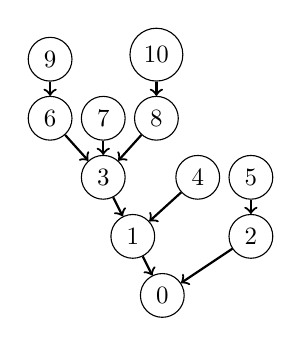
\begin{tikzpicture}[scale=.5, anchor=south]
      \node[circle, scale=0.9, draw] (tid0) at (3,1.5){0};
      \node[circle, scale=0.9, draw] (tid1) at (2.25,3){1};
      \node[circle, scale=0.9, draw] (tid2) at (1.5,4.5){3};
      \node[circle, scale=0.9, draw] (tid7) at (0.15,6){6};
      \node[circle, scale=0.9, draw] (tid9) at (0.15,7.5){9};
      \draw[<-, thick](tid7) -- (tid9);
      \node[circle, scale=0.9, draw] (tid10) at (1.5,6){7};
      \draw[<-, thick](tid2) -- (tid7);
      \draw[<-, thick](tid2) -- (tid10);
      \node[circle, scale=0.9, draw] (tid3) at (3.9,4.5){4};
      \node[circle, scale=0.9, draw] (tid5) at (2.85,6){8};
      \node[circle, scale=0.9, draw] (tid6) at (2.85,7.5){10
};
      \draw[<-, thick](tid5) -- (tid6);
      \draw[<-, thick](tid2) -- (tid5);
      \draw[<-, thick](tid1) -- (tid2);
      \draw[<-, thick](tid1) -- (tid3);
      \node[circle, scale=0.9, draw] (tid4) at (5.25,3){2};
      \node[circle, scale=0.9, draw] (tid8) at (5.25,4.5){5};
      \draw[<-, thick](tid4) -- (tid8);
      \draw[<-, thick](tid0) -- (tid1);
      \draw[<-, thick](tid0) -- (tid4);
    \end{tikzpicture}
  \end{center}
\end{frame}

\todo{Nonpreemtiv, etc (precise problem description!)}

\subsection{Schedules}
\label{sec:schedules}

\begin{frame}
  \frametitle{Schedules}
  \begin{itemize}
  \item A schedule describes the order in which tasks are processed
  \item Non-deterministic in our scenario (task times are random variables)
  \item Scheduling strategy influences expected make span
  \end{itemize}
\end{frame}

\begin{frame}
  \frametitle{Snapshots}
  \begin{itemize}
  \item Each state of a schedule is a snapshot
  \item Snapshot consists current intree and set of scheduled tasks
  \item A schedule can be visualized by a snapshot DAG
  \end{itemize}
\end{frame}

\begin{frame}
  \frametitle{Schedule visualization}
  \only<1>{
    \begin{center}
      \renewcommand{\leveltopI}{-15cm + \leveltop}
\renewcommand{\leveltopII}{-15cm + \leveltopI}
\renewcommand{\leveltopIII}{-16cm + \leveltopII}
\renewcommand{\leveltopIIII}{-12cm + \leveltopIII}
\renewcommand{\leveltopIIIII}{-12cm + \leveltopIIII}
\renewcommand{\leveltopIIIIII}{-12cm + \leveltopIIIII}
\renewcommand{\leveltopIIIIIII}{-12cm + \leveltopIIIIII}
\renewcommand{\leveltopIIIIIIII}{-12cm + \leveltopIIIIIII}
\renewcommand{\leveltopIIIIIIIII}{-12cm + \leveltopIIIIIIII}
\renewcommand{\leveltopIIIIIIIIII}{-12cm + \leveltopIIIIIIIII}
\renewcommand{\leveltopIIIIIIIIIII}{-12cm + \leveltopIIIIIIIIII}
\begin{tikzpicture}[scale=.13333, anchor=south]
  % legende
  \filldraw[dashed,fill=gray!10!white] (-20, -30) rectangle +(36.5, 12);
  % \draw[dashed] (-30, -13) -- +(60, 0);
  % \draw[dashed] (-30, -24) -- +(60, 0);
  % \node at (10, -21) {Intermediate snapshots};
  \begin{scope}[yshift=\leveltopI cm]
    \matrix (line1)[column sep=0.5cm, ampersand replacement=\&] {
      \node[draw=black, rectangle split,  rectangle split parts=1] (sn0x17d67b0){
        \begin{tikzpicture}[scale=.13333]
          \node[circle, scale=0.5, fill] (tid0) at (4.5,1.5){};
          \node[circle, scale=0.5, fill] (tid2) at (2.25,3){};
          \node[circle, scale=0.5, fill, task_scheduled] (tid4) at (2.25,4.5){};
          \draw[](tid2) -- (tid4);
          \node[circle, scale=0.5, fill] (tid3) at (6,3){};
          \node[circle, scale=0.5, fill] (tid5) at (3.75,4.5){};
          \node[circle, scale=0.5, fill] (tid6) at (5.25,4.5){};
          \node[circle, scale=0.5, fill] (tid7) at (7.5,4.5){};
          \node[circle, scale=0.5, fill] (tid8) at (6.75,6){};
          \node[circle, scale=0.5, fill] (tid9) at (8.25,6){};
          \node[circle, scale=0.5, fill, task_scheduled] (tid10) at (8.25,7.5){};
          \draw[](tid9) -- (tid10);
          \draw[](tid7) -- (tid8);
          \draw[](tid7) -- (tid9);
          \draw[](tid3) -- (tid5);
          \draw[](tid3) -- (tid6);
          \draw[](tid3) -- (tid7);
          \draw[](tid0) -- (tid2);
          \draw[](tid0) -- (tid3);
        \end{tikzpicture}
      }
      ;
      \& 
      \\
    };
  \end{scope}
  \begin{scope}[yshift=\leveltopII cm]
    \matrix (line2)[column sep=0.5cm, ampersand replacement=\&] {
      \node[draw=black, rectangle split,  rectangle split parts=1] (sn0x17d65a0){
        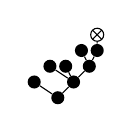
\begin{tikzpicture}[scale=.13333]
          \node[circle, scale=0.5, fill] (tid0) at (4.5,1.5){};
          \node[circle, scale=0.5, fill] (tid2) at (2.25,3){};
          \node[circle, scale=0.5, fill] (tid3) at (6,3){};
          \node[circle, scale=0.5, fill] (tid5) at (3.75,4.5){};
          \node[circle, scale=0.5, fill] (tid6) at (5.25,4.5){};
          \node[circle, scale=0.5, fill] (tid7) at (7.5,4.5){};
          \node[circle, scale=0.5, fill] (tid8) at (6.75,6){};
          \node[circle, scale=0.5, fill] (tid9) at (8.25,6){};
          \node[circle, scale=0.5, fill, task_scheduled] (tid10) at (8.25,7.5){};
          \draw[](tid9) -- (tid10);
          \draw[](tid7) -- (tid8);
          \draw[](tid7) -- (tid9);
          \draw[](tid3) -- (tid5);
          \draw[](tid3) -- (tid6);
          \draw[](tid3) -- (tid7);
          \draw[](tid0) -- (tid2);
          \draw[](tid0) -- (tid3);
        \end{tikzpicture}
      }
      ;
      \& 
      \node[minimum width=1cm]{};
      \&
      \node[draw=black, rectangle split,  rectangle split parts=1] (sn0x17d57c0){
        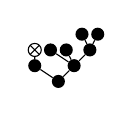
\begin{tikzpicture}[scale=.13333]
          \node[circle, scale=0.5, fill] (tid0) at (4.5,1.5){};
          \node[circle, scale=0.5, fill] (tid2) at (2.25,3){};
          \node[circle, scale=0.5, fill, task_scheduled] (tid4) at (2.25,4.5){};
          \draw[](tid2) -- (tid4);
          \node[circle, scale=0.5, fill] (tid3) at (6,3){};
          \node[circle, scale=0.5, fill] (tid5) at (3.75,4.5){};
          \node[circle, scale=0.5, fill] (tid6) at (5.25,4.5){};
          \node[circle, scale=0.5, fill] (tid7) at (7.5,4.5){};
          \node[circle, scale=0.5, fill] (tid8) at (6.75,6){};
          \node[circle, scale=0.5, fill] (tid9) at (8.25,6){};
          \draw[](tid7) -- (tid8);
          \draw[](tid7) -- (tid9);
          \draw[](tid3) -- (tid5);
          \draw[](tid3) -- (tid6);
          \draw[](tid3) -- (tid7);
          \draw[](tid0) -- (tid2);
          \draw[](tid0) -- (tid3);
        \end{tikzpicture}
      }
      ;
      \& 
      \\
    };
  \end{scope}
  \begin{scope}[yshift=\leveltopIII cm]
    \matrix (line3)[column sep=0.5cm, ampersand replacement=\&] {
      \node[draw=black, rectangle split,  rectangle split parts=1] (sn0x17d55b0){
        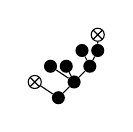
\begin{tikzpicture}[scale=.13333]
          \node[circle, scale=0.5, fill] (tid0) at (4.5,1.5){};
          \node[circle, scale=0.5, fill, task_scheduled] (tid2) at (2.25,3){};
          \node[circle, scale=0.5, fill] (tid3) at (6,3){};
          \node[circle, scale=0.5, fill] (tid5) at (3.75,4.5){};
          \node[circle, scale=0.5, fill] (tid6) at (5.25,4.5){};
          \node[circle, scale=0.5, fill] (tid7) at (7.5,4.5){};
          \node[circle, scale=0.5, fill] (tid8) at (6.75,6){};
          \node[circle, scale=0.5, fill] (tid9) at (8.25,6){};
          \node[circle, scale=0.5, fill, task_scheduled] (tid10) at (8.25,7.5){};
          \draw[](tid9) -- (tid10);
          \draw[](tid7) -- (tid8);
          \draw[](tid7) -- (tid9);
          \draw[](tid3) -- (tid5);
          \draw[](tid3) -- (tid6);
          \draw[](tid3) -- (tid7);
          \draw[](tid0) -- (tid2);
          \draw[](tid0) -- (tid3);
        \end{tikzpicture}
      }
      ;
      \& 
      \node[draw=black, rectangle split,  rectangle split parts=1] (sn0x17d6160){
        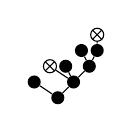
\begin{tikzpicture}[scale=.13333]
          \node[circle, scale=0.5, fill] (tid0) at (4.5,1.5){};
          \node[circle, scale=0.5, fill] (tid2) at (2.25,3){};
          \node[circle, scale=0.5, fill] (tid3) at (6,3){};
          \node[circle, scale=0.5, fill, task_scheduled] (tid5) at (3.75,4.5){};
          \node[circle, scale=0.5, fill] (tid6) at (5.25,4.5){};
          \node[circle, scale=0.5, fill] (tid7) at (7.5,4.5){};
          \node[circle, scale=0.5, fill] (tid8) at (6.75,6){};
          \node[circle, scale=0.5, fill] (tid9) at (8.25,6){};
          \node[circle, scale=0.5, fill, task_scheduled] (tid10) at (8.25,7.5){};
          \draw[](tid9) -- (tid10);
          \draw[](tid7) -- (tid8);
          \draw[](tid7) -- (tid9);
          \draw[](tid3) -- (tid5);
          \draw[](tid3) -- (tid6);
          \draw[](tid3) -- (tid7);
          \draw[](tid0) -- (tid2);
          \draw[](tid0) -- (tid3);
        \end{tikzpicture}
      }
      ;
      \& 
      \node[draw=black, rectangle split,  rectangle split parts=1] (sn0x17d5380){
        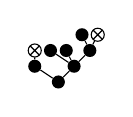
\begin{tikzpicture}[scale=.13333]
          \node[circle, scale=0.5, fill] (tid0) at (4.5,1.5){};
          \node[circle, scale=0.5, fill] (tid2) at (2.25,3){};
          \node[circle, scale=0.5, fill, task_scheduled] (tid4) at (2.25,4.5){};
          \draw[](tid2) -- (tid4);
          \node[circle, scale=0.5, fill] (tid3) at (6,3){};
          \node[circle, scale=0.5, fill] (tid5) at (3.75,4.5){};
          \node[circle, scale=0.5, fill] (tid6) at (5.25,4.5){};
          \node[circle, scale=0.5, fill] (tid7) at (7.5,4.5){};
          \node[circle, scale=0.5, fill] (tid8) at (6.75,6){};
          \node[circle, scale=0.5, fill, task_scheduled] (tid9) at (8.25,6){};
          \draw[](tid7) -- (tid8);
          \draw[](tid7) -- (tid9);
          \draw[](tid3) -- (tid5);
          \draw[](tid3) -- (tid6);
          \draw[](tid3) -- (tid7);
          \draw[](tid0) -- (tid2);
          \draw[](tid0) -- (tid3);
        \end{tikzpicture}
      }
      ;
      \& 
      \node[draw=black, rectangle split,  rectangle split parts=1] (sn0x17d2f50){
        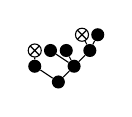
\begin{tikzpicture}[scale=.13333]
          \node[circle, scale=0.5, fill] (tid0) at (4.5,1.5){};
          \node[circle, scale=0.5, fill] (tid2) at (2.25,3){};
          \node[circle, scale=0.5, fill, task_scheduled] (tid4) at (2.25,4.5){};
          \draw[](tid2) -- (tid4);
          \node[circle, scale=0.5, fill] (tid3) at (6,3){};
          \node[circle, scale=0.5, fill] (tid5) at (3.75,4.5){};
          \node[circle, scale=0.5, fill] (tid6) at (5.25,4.5){};
          \node[circle, scale=0.5, fill] (tid7) at (7.5,4.5){};
          \node[circle, scale=0.5, fill, task_scheduled] (tid8) at (6.75,6){};
          \node[circle, scale=0.5, fill] (tid9) at (8.25,6){};
          \draw[](tid7) -- (tid8);
          \draw[](tid7) -- (tid9);
          \draw[](tid3) -- (tid5);
          \draw[](tid3) -- (tid6);
          \draw[](tid3) -- (tid7);
          \draw[](tid0) -- (tid2);
          \draw[](tid0) -- (tid3);
        \end{tikzpicture}
      }
      ;
      \& 
      \node[draw=black, rectangle split,  rectangle split parts=1] (sn0x17d3a00){
        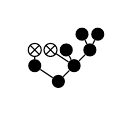
\begin{tikzpicture}[scale=.13333]
          \node[circle, scale=0.5, fill] (tid0) at (4.5,1.5){};
          \node[circle, scale=0.5, fill] (tid2) at (2.25,3){};
          \node[circle, scale=0.5, fill, task_scheduled] (tid4) at (2.25,4.5){};
          \draw[](tid2) -- (tid4);
          \node[circle, scale=0.5, fill] (tid3) at (6,3){};
          \node[circle, scale=0.5, fill, task_scheduled] (tid5) at (3.75,4.5){};
          \node[circle, scale=0.5, fill] (tid6) at (5.25,4.5){};
          \node[circle, scale=0.5, fill] (tid7) at (7.5,4.5){};
          \node[circle, scale=0.5, fill] (tid8) at (6.75,6){};
          \node[circle, scale=0.5, fill] (tid9) at (8.25,6){};
          \draw[](tid7) -- (tid8);
          \draw[](tid7) -- (tid9);
          \draw[](tid3) -- (tid5);
          \draw[](tid3) -- (tid6);
          \draw[](tid3) -- (tid7);
          \draw[](tid0) -- (tid2);
          \draw[](tid0) -- (tid3);
        \end{tikzpicture}
      }
      ;
      \& 
      \\
    };
  \end{scope}
  \draw (sn0x17d67b0.south) -- node[xshift=.4cm]{$0.5$} (sn0x17d57c0.north);
  \draw (sn0x17d67b0.south) -- node[left, yshift=.2cm]{$0.5$} (sn0x17d65a0.north);
  \draw (sn0x17d65a0.south) -- node[right]{$0.8$} (sn0x17d6160.north);
  \draw (sn0x17d65a0.south) -- node[left, xshift=-.25cm]{$0.2$} (sn0x17d55b0.north);
  \draw (sn0x17d57c0.south) -- node[right, xshift=.25]{$0.2$} (sn0x17d2f50.north);
  \draw (sn0x17d57c0.south) -- node[left, xshift=-3]{$0.4$} (sn0x17d5380.north);
  \draw (sn0x17d57c0.south) -- node[right, xshift=5]{$0.4$} (sn0x17d3a00.north);
\end{tikzpicture} % with intermediate snaps
    \end{center}
  }
  \only<2>{
    \begin{center}
      \input{talk_schedule_vis2} % without intermediate snaps
    \end{center}
  }
  \only<3>{
    \begin{center}
      \input{talk_schedule_vis3} % compressed form
    \end{center}
  }
\end{frame}

\begin{frame}
  \frametitle{Epected run time}
  \begin{itemize}
  \item $r$ tasks currently scheduled
  \item Compute run time recursively:
    \begin{itemize}
    \item Expected time for fastest task ($\frac{1}{r}$)
    \item Weighted expected time for successive snapshots
    \end{itemize}
  \end{itemize}
\end{frame}

\begin{frame}
  \only<1>{
    \begin{center}
      \input{talk_schedule_vis3} % compressed form
    \end{center}
  }
  \only<2>{
    \begin{center}
      \renewcommand{\leveltopI}{-25cm + \leveltop}
\renewcommand{\leveltopII}{-25cm + \leveltopI}
\renewcommand{\leveltopIII}{-16cm + \leveltopII}
\renewcommand{\leveltopIIII}{-12cm + \leveltopIII}
\renewcommand{\leveltopIIIII}{-12cm + \leveltopIIII}
\renewcommand{\leveltopIIIIII}{-12cm + \leveltopIIIII}
\renewcommand{\leveltopIIIIIII}{-12cm + \leveltopIIIIII}
\renewcommand{\leveltopIIIIIIII}{-12cm + \leveltopIIIIIII}
\renewcommand{\leveltopIIIIIIIII}{-12cm + \leveltopIIIIIIII}
\renewcommand{\leveltopIIIIIIIIII}{-12cm + \leveltopIIIIIIIII}
\renewcommand{\leveltopIIIIIIIIIII}{-12cm + \leveltopIIIIIIIIII}
\begin{tikzpicture}[scale=.13333, anchor=south]
  % legende
  %\filldraw[dashed,fill=gray!10!white] (-20, -30) rectangle +(36.5, 12);
  % \draw[dashed] (-30, -13) -- +(60, 0);
  % \draw[dashed] (-30, -24) -- +(60, 0);
  % \node at (10, -21) {Intermediate snapshots};
  \begin{scope}[yshift=\leveltopI cm]
    \matrix (line1)[column sep=0.5cm, ampersand replacement=\&] {
      \node[draw=black, rectangle split,  rectangle split parts=3] (sn0x17d67b0){
        \begin{tikzpicture}[scale=.13333]
          \node[circle, scale=0.5, fill] (tid0) at (4.5,1.5){};
          \node[circle, scale=0.5, fill] (tid2) at (2.25,3){};
          \node[circle, scale=0.5, fill, task_scheduled] (tid4) at (2.25,4.5){};
          \draw[](tid2) -- (tid4);
          \node[circle, scale=0.5, fill] (tid3) at (6,3){};
          \node[circle, scale=0.5, fill] (tid5) at (3.75,4.5){};
          \node[circle, scale=0.5, fill] (tid6) at (5.25,4.5){};
          \node[circle, scale=0.5, fill] (tid7) at (7.5,4.5){};
          \node[circle, scale=0.5, fill] (tid8) at (6.75,6){};
          \node[circle, scale=0.5, fill] (tid9) at (8.25,6){};
          \node[circle, scale=0.5, fill, task_scheduled] (tid10) at (8.25,7.5){};
          \draw[](tid9) -- (tid10);
          \draw[](tid7) -- (tid8);
          \draw[](tid7) -- (tid9);
          \draw[](tid3) -- (tid5);
          \draw[](tid3) -- (tid6);
          \draw[](tid3) -- (tid7);
          \draw[](tid0) -- (tid2);
          \draw[](tid0) -- (tid3);
        \end{tikzpicture}
        \nodepart{second}
        ? %6.43745
        \nodepart{third}
        \footnotesize{10\ 40\ 20\ 10\ 20}
      }
      ;
      \& 
      \\
    };
  \end{scope}
  \begin{scope}[yshift=\leveltopII cm]
    \matrix (line2)[column sep=.5cm, ampersand replacement=\&] {
      \node[draw=black, rectangle split,  rectangle split parts=2] (sn0x17d55b0){
        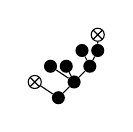
\begin{tikzpicture}[scale=.13333]
          \node[circle, scale=0.5, fill] (tid0) at (4.5,1.5){};
          \node[circle, scale=0.5, fill, task_scheduled] (tid2) at (2.25,3){};
          \node[circle, scale=0.5, fill] (tid3) at (6,3){};
          \node[circle, scale=0.5, fill] (tid5) at (3.75,4.5){};
          \node[circle, scale=0.5, fill] (tid6) at (5.25,4.5){};
          \node[circle, scale=0.5, fill] (tid7) at (7.5,4.5){};
          \node[circle, scale=0.5, fill] (tid8) at (6.75,6){};
          \node[circle, scale=0.5, fill] (tid9) at (8.25,6){};
          \node[circle, scale=0.5, fill, task_scheduled] (tid10) at (8.25,7.5){};
          \draw[](tid9) -- (tid10);
          \draw[](tid7) -- (tid8);
          \draw[](tid7) -- (tid9);
          \draw[](tid3) -- (tid5);
          \draw[](tid3) -- (tid6);
          \draw[](tid3) -- (tid7);
          \draw[](tid0) -- (tid2);
          \draw[](tid0) -- (tid3);
        \end{tikzpicture}
        \nodepart{second}
        6.1640
      }
      ;
      \& 
      \node[draw=black, rectangle split,  rectangle split parts=2] (sn0x17d6160){
        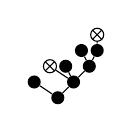
\begin{tikzpicture}[scale=.13333]
          \node[circle, scale=0.5, fill] (tid0) at (4.5,1.5){};
          \node[circle, scale=0.5, fill] (tid2) at (2.25,3){};
          \node[circle, scale=0.5, fill] (tid3) at (6,3){};
          \node[circle, scale=0.5, fill, task_scheduled] (tid5) at (3.75,4.5){};
          \node[circle, scale=0.5, fill] (tid6) at (5.25,4.5){};
          \node[circle, scale=0.5, fill] (tid7) at (7.5,4.5){};
          \node[circle, scale=0.5, fill] (tid8) at (6.75,6){};
          \node[circle, scale=0.5, fill] (tid9) at (8.25,6){};
          \node[circle, scale=0.5, fill, task_scheduled] (tid10) at (8.25,7.5){};
          \draw[](tid9) -- (tid10);
          \draw[](tid7) -- (tid8);
          \draw[](tid7) -- (tid9);
          \draw[](tid3) -- (tid5);
          \draw[](tid3) -- (tid6);
          \draw[](tid3) -- (tid7);
          \draw[](tid0) -- (tid2);
          \draw[](tid0) -- (tid3);
        \end{tikzpicture}
        \nodepart{second}
        5.9921
      }
      ;
      \& 
      \node[draw=black, rectangle split,  rectangle split parts=2] (sn0x17d5380){
        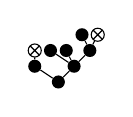
\begin{tikzpicture}[scale=.13333]
          \node[circle, scale=0.5, fill] (tid0) at (4.5,1.5){};
          \node[circle, scale=0.5, fill] (tid2) at (2.25,3){};
          \node[circle, scale=0.5, fill, task_scheduled] (tid4) at (2.25,4.5){};
          \draw[](tid2) -- (tid4);
          \node[circle, scale=0.5, fill] (tid3) at (6,3){};
          \node[circle, scale=0.5, fill] (tid5) at (3.75,4.5){};
          \node[circle, scale=0.5, fill] (tid6) at (5.25,4.5){};
          \node[circle, scale=0.5, fill] (tid7) at (7.5,4.5){};
          \node[circle, scale=0.5, fill] (tid8) at (6.75,6){};
          \node[circle, scale=0.5, fill, task_scheduled] (tid9) at (8.25,6){};
          \draw[](tid7) -- (tid8);
          \draw[](tid7) -- (tid9);
          \draw[](tid3) -- (tid5);
          \draw[](tid3) -- (tid6);
          \draw[](tid3) -- (tid7);
          \draw[](tid0) -- (tid2);
          \draw[](tid0) -- (tid3);
        \end{tikzpicture}
        \nodepart{second}
        5.8203
      }
      ;
      \& 
      \node[draw=black, rectangle split,  rectangle split parts=2] (sn0x17d2f50){
        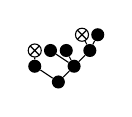
\begin{tikzpicture}[scale=.13333]
          \node[circle, scale=0.5, fill] (tid0) at (4.5,1.5){};
          \node[circle, scale=0.5, fill] (tid2) at (2.25,3){};
          \node[circle, scale=0.5, fill, task_scheduled] (tid4) at (2.25,4.5){};
          \draw[](tid2) -- (tid4);
          \node[circle, scale=0.5, fill] (tid3) at (6,3){};
          \node[circle, scale=0.5, fill] (tid5) at (3.75,4.5){};
          \node[circle, scale=0.5, fill] (tid6) at (5.25,4.5){};
          \node[circle, scale=0.5, fill] (tid7) at (7.5,4.5){};
          \node[circle, scale=0.5, fill, task_scheduled] (tid8) at (6.75,6){};
          \node[circle, scale=0.5, fill] (tid9) at (8.25,6){};
          \draw[](tid7) -- (tid8);
          \draw[](tid7) -- (tid9);
          \draw[](tid3) -- (tid5);
          \draw[](tid3) -- (tid6);
          \draw[](tid3) -- (tid7);
          \draw[](tid0) -- (tid2);
          \draw[](tid0) -- (tid3);
        \end{tikzpicture}
        \nodepart{second}
        5.8203
      }
      ;
      \& 
      \node[draw=black, rectangle split,  rectangle split parts=2] (sn0x17d3a00){
        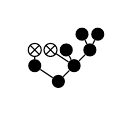
\begin{tikzpicture}[scale=.13333]
          \node[circle, scale=0.5, fill] (tid0) at (4.5,1.5){};
          \node[circle, scale=0.5, fill] (tid2) at (2.25,3){};
          \node[circle, scale=0.5, fill, task_scheduled] (tid4) at (2.25,4.5){};
          \draw[](tid2) -- (tid4);
          \node[circle, scale=0.5, fill] (tid3) at (6,3){};
          \node[circle, scale=0.5, fill, task_scheduled] (tid5) at (3.75,4.5){};
          \node[circle, scale=0.5, fill] (tid6) at (5.25,4.5){};
          \node[circle, scale=0.5, fill] (tid7) at (7.5,4.5){};
          \node[circle, scale=0.5, fill] (tid8) at (6.75,6){};
          \node[circle, scale=0.5, fill] (tid9) at (8.25,6){};
          \draw[](tid7) -- (tid8);
          \draw[](tid7) -- (tid9);
          \draw[](tid3) -- (tid5);
          \draw[](tid3) -- (tid6);
          \draw[](tid3) -- (tid7);
          \draw[](tid0) -- (tid2);
          \draw[](tid0) -- (tid3);
        \end{tikzpicture}
        \nodepart{second}
        5.8906
      }
      ;
      \& 
      \\
    };
  \end{scope}
  \draw (sn0x17d67b0.south) -- (sn0x17d6160.north);
  \draw (sn0x17d67b0.south) -- (sn0x17d55b0.north);
  \draw (sn0x17d67b0.south) -- (sn0x17d2f50.north);
  \draw (sn0x17d67b0.south) -- (sn0x17d5380.north);
  \draw (sn0x17d67b0.south) -- (sn0x17d3a00.north);
  \draw[decorate, decoration=brace] (sn0x17d3a00.north) ++ (0,14) --node [right]{Exp. $\frac{1}{2}$} ++ (0,-13); 
\end{tikzpicture} % expected run times
    \end{center}
  }
  \begin{equation*}
    \frac{1}{2}
    + 0.1 \cdot 6.1640
    + 0.4 \cdot 5.9921
    + 0.2 \cdot 5.8203
    + \dots
    % + 0.1 \cdot 5.8203
    % + 0.2 \cdot 5.8906
    = 6.43745
  \end{equation*}
\end{frame}

\begin{frame}
  \frametitle{Equivalent snapshots}
  \begin{itemize}
  \item The following two snapshots (basically) describe the same problem:
  \end{itemize}
\end{frame}

\end{document}

%%% Local Variables: 
%%% mode: latex
%%% TeX-master: t
%%% End: 
